\documentclass[11pt,letterpaper]{article}
\usepackage[T1]{fontenc}
\usepackage{lmodern}
\usepackage[margin=0.94in,top=0.86in,bottom=0.86in,headheight=15pt,headsep=16pt]{geometry}
\usepackage{amsmath,amssymb,booktabs,graphicx,microtype,fancyhdr,xcolor}
\definecolor{ink}{HTML}{183F4B}
\definecolor{muted}{HTML}{465D65}
\usepackage[font=small,labelfont={bf,color=ink},labelsep=period,
            justification=raggedright,singlelinecheck=false,skip=5pt]{caption}
\usepackage[hidelinks,bookmarksnumbered]{hyperref}
\graphicspath{{figures/}{../report/evidence/}}
\providecommand{\TeamNumber}{720}
\hypersetup{pdftitle={Predicting Penalty Trajectories: What Two Early Positions Can Resolve},pdfauthor={},pdflang={en}}
\pagestyle{fancy}
\fancyhf{}
\fancyhead[R]{\small\sffamily\color{muted}Team \TeamNumber}
\fancyfoot[C]{\small\sffamily\color{muted}\thepage}
\renewcommand{\headrulewidth}{0.3pt}
\fancypagestyle{cover}{\fancyhf{}\fancyhead[R]{\small\sffamily\color{muted}Team \TeamNumber}\renewcommand{\headrulewidth}{0pt}}
\makeatletter
\renewcommand{\section}{\@startsection{section}{1}{\z@}
  {-2.5ex \@plus -.4ex \@minus -.2ex}{1.2ex \@plus .2ex}
  {\normalfont\Large\bfseries\color{ink}\raggedright}}
\renewcommand{\subsection}{\@startsection{subsection}{2}{\z@}
  {-1.7ex \@plus -.3ex \@minus -.2ex}{0.55ex \@plus .1ex}
  {\normalfont\normalsize\sffamily\bfseries\color{ink}\raggedright}}
\renewcommand{\@seccntformat}[1]{\csname the#1\endcsname\hspace{.65em}}
\makeatother
\renewenvironment{abstract}
  {\par\noindent{\large\bfseries\color{ink}Abstract}\par\vspace{5pt}\noindent\ignorespaces}
  {\par}
\linespread{1.075}
\setlength{\parindent}{1.15em}
\setlength{\parskip}{2pt plus 0.5pt minus 0.5pt}
\setlength{\textfloatsep}{11pt}
\setlength{\intextsep}{9pt}
\setlength{\emergencystretch}{1em}
\raggedbottom
\renewcommand{\topfraction}{.88}
\renewcommand{\textfraction}{.10}
\renewcommand{\floatpagefraction}{.73}
\setcounter{topnumber}{3}
\newcommand{\vv}[1]{\boldsymbol{#1}}
\newcommand{\norm}[1]{\lVert #1\rVert}
\newcommand{\doi}[1]{\href{https://doi.org/#1}{\nolinkurl{#1}}}
\newcommand{\reserveheadroom}{\par\ifdim\dimexpr\pagegoal-\pagetotal\relax<5\baselineskip\newpage\fi}

\begin{document}
\thispagestyle{cover}
\vspace*{0.60in}
\begin{center}
\begin{minipage}{0.89\textwidth}
\raggedright
{\large\sffamily\bfseries\color{muted}Problem B\par}
\vspace{0.25in}
{\fontsize{25}{30}\selectfont\bfseries\color{ink}
 Predicting Penalty Trajectories:\\
 What Two Early Positions\\
 Can Resolve\par}
\vspace{0.28in}
{\color{muted}\hrule height 0.45pt}
\vspace{0.24in}
\pdfbookmark[1]{Abstract}{cover-abstract}
\begin{abstract}
\leftskip=0pt \rightskip=0pt \parfillskip=0pt plus 1fil
We use the ball's positions 50 and 100 ms after release to estimate the probability of direct entry and the most likely point of entry on the goal plane. For the prescribed kick, assuming exact release timing, centimetre rounding and horizontal wind speeds up to 3 m/s, the most probable cell is centred at \((Y,Z)=(2.56,2.07)\) m. Six cells covering \(0.3572\ \mathrm{m^2}\) contain 90.52\% of the model probability conditional on direct entry. The median crossing time is 0.399 s. Two admissible flights reproduce the same readings and cross 8.76 cm apart. For this pair the worst-case error of any point forecast is at least about 4.38 cm.

We calibrated prediction regions on 90 synthetic kicks and tested them on 120 others, of which 71 entered directly. With rounding alone, the two-frame and late-frame aerodynamic forecasts both covered 70 of 71 entries at their 95\% calibration targets. Their regions averaged 0.585 and 3.482 \(\mathrm{m^2}\), respectively. A two-frame gravity model covered the same number in 1.222 \(\mathrm{m^2}\). Adding the 50 ms reading reduced mean point error by 3.80 cm relative to the late frame alone. With 6 mm independent and 8 mm shared tracking errors, both gravity and two-frame aerodynamics covered 67 of 71, at calibration targets of 80\% and 95\%, respectively. Gravity used 0.933 \(\mathrm{m^2}\); aerodynamics used 1.385 \(\mathrm{m^2}\). The three available match records lacked an independent release time, so accuracy on real penalties remains open.
\end{abstract}
\end{minipage}
\end{center}
\clearpage

\section{What the first 100 ms reveal about the flight}

At 100 ms the ball in the prescribed penalty has travelled only 2.96 m toward the goal. The two readings reveal its average velocity over the preceding 50 ms, yet the crossing depends on how drag and transverse forces act over the remaining 8.04 m (Fig.~\ref{fig:geometry}). The task is to predict where the ball is most likely to enter the goal, estimate the uncertainty in that location and test the method~\cite{upc}.


We first ask which forces can explain the early positions. We then follow the admissible flights to their first event. This gives the probability of direct entry and, among flights that enter, a point and joint region on the goal plane (Table~\ref{tab:taskmap}). The problem supplies no final position for the prescribed kick, so we assess accuracy on separate kicks.

\begin{figure}[htbp]\centering
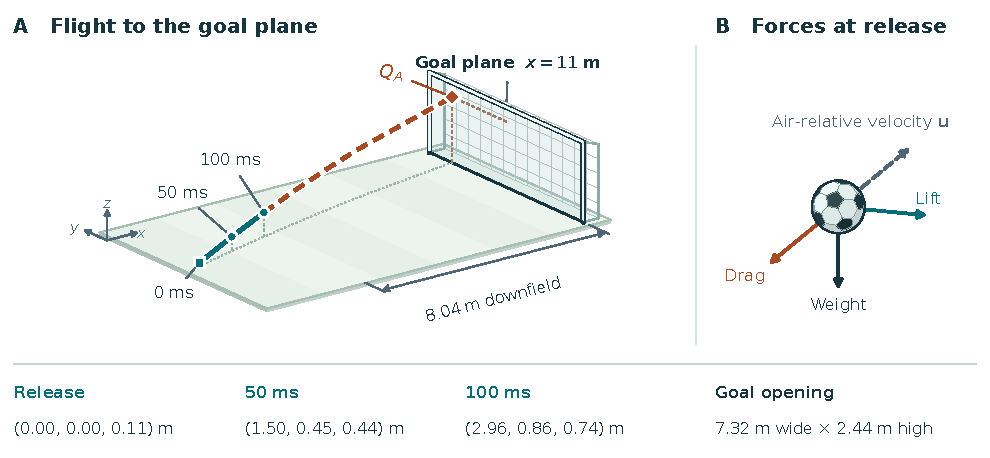
\includegraphics[width=\linewidth]{problem-geometry.pdf}
\caption{\textbf{Two readings and one admissible flight.} In A, the square marks release and the circles mark the prescribed ball centres, given below in $(x,y,z)$ order. Dashed segments join archived positions of flight A to its crossing $Q_A$ (Sec.~\ref{sec:ambig}). The dotted line on the turf is the ground projection. B shows the same flight at release in still air. Drag opposes the air-relative velocity, lift acts perpendicular to it in three dimensions, and weight points down. Arrow lengths are schematic.}
\label{fig:geometry}
\end{figure}

\begin{table}[htbp]\centering\small
\caption{How the two observations available by 100 ms enter each part of the problem.}
\label{tab:taskmap}
\begin{tabular}{@{}p{.30\linewidth}p{.40\linewidth}p{.22\linewidth}@{}}\toprule
Task & Forecast or test & Evidence\\\midrule
Develop a predictor & First-event probabilities and highest-mass goal cell & Eqs.~\eqref{eq:acc}, \eqref{eq:weights}\\
Estimate uncertainty & Joint region and sensitivity to observation and force assumptions & Figs.~\ref{fig:goal}--\ref{fig:sensitivity}\\
Apply and test & Prescribed kick and synthetic kicks at the same 100 ms cutoff & Eq.~\eqref{eq:region}, Fig.~\ref{fig:frontier}\\
\bottomrule\end{tabular}
\end{table}

\subsection{Observations and possible outcomes}
Let \(x\) point from the penalty spot toward the goal, \(y\) run across its face and \(z\) measure height above the ground. The ball centre starts at \(\vv r_0=(0,0,0.11)\) m. Its two prescribed positions, in metres, are
\begin{equation}
 \vv r(0.050\,\mathrm{s})=(1.50,0.45,0.44),\qquad
 \vv r(0.100\,\mathrm{s})=(2.96,0.86,0.74).
 \label{eq:data}
\end{equation}
For the reference forecast we take the release position and observation times as exact and interpret the displayed coordinates as rounded to the nearest centimetre. Each later coordinate \(q\) then represents \([q-\epsilon,q+\epsilon)\), with \(\epsilon=0.005\) m. The problem supplies no tracking accuracy, ball type, wind or spin. Section~\ref{sec:measurement} examines how different observation assumptions affect this kick.

We follow the ball to its first forward crossing of \(x=11\) m or its first descent to one ball radius above ground. A direct entry \(G\) occurs when the centre crosses the 7.32 m wide opening with \(-3.66<Y<3.66\) m and \(0<Z<2.44\) m. The other outcomes are a crossing outside the opening, earlier ground contact, or neither event by 1.25 s. We estimate all four probabilities and the distribution of \(Q=(Y,Z)\) conditional on \(G\). This ball-centre convention omits frame collisions, rebounds and goalkeeper interventions.

\subsection{How much wind would drag alone require?}
The mean horizontal velocities over the first and second 50 ms are \((30.0,9.0)\) and \((29.2,8.2)\) m/s. Their directions differ. Under drag alone in a constant horizontal wind \(\vv w\), the horizontal velocity keeps its direction relative to the air. The horizontal displacements \(\vv p_i\) from release must therefore satisfy
\begin{equation}
 \det(\vv p_1-t_1\vv w,\,\vv p_2-t_2\vv w)=0,
 \qquad
 \norm{\vv w}\ge
 \frac{|\det(\vv p_1,\vv p_2)|}{\norm{t_2\vv p_1-t_1\vv p_2}} .
 \label{eq:wind}
\end{equation}
Treating the displayed positions as exact gives a minimum wind speed of 14.849 m/s. For fixed wind the determinant, the signed area spanned by the two vectors, is linear in each coordinate separately. Its extrema on the closed rounding boxes therefore occur at their corners. Allowing for rounding lowers the infimum to 4.353 m/s, still above the 3 m/s wind cap. Under this cap the kick requires a transverse force, but the observations leave its source open. A wind that passes the collinearity test must still satisfy the full flight equations.

In still air the horizontal path under drag alone must be a straight line through the origin. For the positive coordinates in this example, the closure of the slope interval from frame \(i\) is
\[
 \left[\frac{y_i-\epsilon}{x_i+\epsilon},\,\frac{y_i+\epsilon}{x_i-\epsilon}\right].
\]
The two ranges first touch at \(\epsilon=7.279\) mm. Thus a 5 mm per-coordinate bound resolves a departure from a straight horizontal path. At a 1 cm bound the readings admit such a path.


\section{From aerodynamic forces to a crossing forecast}

\subsection{Three force laws and their parameter ranges}
Write \(\vv v=\dot{\vv r}\) for velocity over the ground, \(\vv u=\vv v-\vv w\) for velocity relative to the air, and \(U=\norm{\vv u}\). The three force models give accelerations
\begin{equation}
\begin{aligned}
 \vv a_{\mathrm D}&=\vv g-\kappa U\vv u,\\
 \vv a_{\mathrm S}&=\vv a_{\mathrm D}+\vv\beta\times\vv u,\\
 \vv a_{\mathrm E}&=\vv g-K C_D U\vv u+K C_L U^2\vv n .
\end{aligned}
\label{eq:acc}
\end{equation}
Model D has quadratic drag. S adds a transverse force with constant coefficient vector \(\vv\beta\). In E, \(K=\rho\pi R^2/(2m)\) and lift acts along the unit vector \(\vv n\) in the direction of \(\vv\omega\times\vv u\). Lift vanishes when the cross product is zero. We use \(g=9.81\ \mathrm{m/s^2}\) downward, radius \(R=0.11\) m, mass \(m=0.43\) kg and air density \(\rho=1.20\ \mathrm{kg/m^3}\). With inputs in SI units, the coefficients for E are
\begin{equation}
\begin{aligned}
 C_D&=0.155+\frac{0.346}{1+\exp[(U_c-12.19)/1.309]}+\delta,\qquad
 U_c=\min(29.9,\max(9.3,U)),\\
 C_L&=0.38\tanh\!\left(5R\norm{\vv\omega\times\vv u}/U^2\right).
\end{aligned}
\label{eq:coeff}
\end{equation}
The drag transition in E comes from a wind-tunnel fit for a nonspinning Teamgeist ball~\cite{goff2010}. We clip its speed argument to 9.3--29.9 m/s, the initial-speed range of a separate 29-flight study~\cite{goff2017}. Extrapolation to the unknown ball remains uncertain. The offset \(\delta\), the saturating lift curve and the broad spin range in E are modelling choices. In S, \(\vv\beta\) is an effective transverse-force coefficient.

We assign D, S and E prior probabilities \(0.2,0.4,0.4\) and draw wind uniformly from a horizontal disk of radius 3 m/s. Launch-velocity components are independently uniform over \([18,38]\), \([-12,12]\) and \([1.5,11]\) m/s along \(x,y,z\). For D and S, \(\kappa\) is uniform on \([0.006,0.024]\ \mathrm{m^{-1}}\). The components of \(\vv\beta\) in S and \(\vv\omega\) in E are uniform within \(\pm0.8\ \mathrm{s^{-1}}\) and \(\pm65\ \mathrm{rad/s}\), respectively. In E, \(\delta\) is uniform on \([-0.04,0.27]\).


\subsection{Force scales over the remaining flight}
The first displacement gives a speed scale \(U_0\simeq32\) m/s. At \(\kappa\simeq0.020\ \mathrm{m^{-1}}\), the 0.4 s flight lasts about 0.26 of the drag time \((\kappa U_0)^{-1}\simeq1.56\) s. A transverse coefficient of \(0.5\ \mathrm{s^{-1}}\) gives an initial acceleration scale of 16 m/s\(^2\). A residual transverse acceleration of 1 m/s\(^2\) sustained over the remaining 0.30 s would accumulate about 4.5 cm of displacement.

Constant wind also gives an energy check. Because \(\vv u\cdot(\vv\beta\times\vv u)=0\) and \(\vv u\cdot\vv n=0\),
\[
 \frac{\mathrm d}{\mathrm dt}\frac{U^2}{2}
   =\vv u\cdot\vv g-d(U)U^2,\qquad d(U)\ge0.
\]
where \(d(U)\) is the nonnegative drag rate. A transverse force turns the air-relative velocity, while drag dissipates air-relative kinetic energy. We use this identity to bound acceleration in the match records.

\subsection{Weighting trajectories and mapping their crossings}
For each draw of wind and aerodynamic parameters, we estimate launch velocity from the latest visible position under gravity and correct the estimate three times by integrating to that position. We draw velocities from a local uniform distribution centred on this estimate, with half-width \(0.007\,\mathrm{m}/t\) per axis at observation time \(t\), or from the original prior with probability 2\%. Under rounding alone, a trajectory inside every observed interval receives the prior-to-proposal density ratio. All others receive zero weight. For parameters \(\theta\), proposal density \(q_M\) and likelihood \(L\),
\begin{equation}
 w_{Mj}=\frac{p(\theta_{Mj}\mid M)L(D\mid\theta_{Mj},M)}{q_M(\theta_{Mj})},\quad
 \widehat Z_M=\frac1{N_M}\sum_jw_{Mj},\quad
 \widehat p(M\mid D)\propto p(M)\widehat Z_M.
 \label{eq:weights}
\end{equation}
Sampling nuisance parameters from their priors cancels those densities in the ratio. The correction for launch velocity remains. The mean weight \(\widehat Z_M\) estimates the evidence for force model \(M\). Systematic resampling limits propagation to 512 trajectories per model per test kick, or 8,192 per model per seed for the prescribed kick. Both prescribed-case runs stayed below their cap.

We use fourth-order Runge--Kutta steps of 25 ms through the two prescribed observations and at most 12.5 ms thereafter. Linear interpolation locates plane crossings and ground contact within a step. Four numerical checks, including independent SciPy DOP853 integrations~\cite{scipy}, agreed within 0.171 mm in event position and 0.038 ms in time.

First-event probabilities use the weights of all trajectories. For direct entries we normalize their weights on a \(30\times10\) equal-area goal grid. The centre of the most probable cell gives the point forecast. Adding cells in decreasing order of probability until they contain at least 90\% gives the raw joint region (Fig.~\ref{fig:workflow}). Zero total weight leaves the forecast undefined. If only the direct-entry weight is zero, we can still report event probabilities. We flag test kicks with an effective sample size \(\mathrm{ESS}=1/\sum_j\bar w_j^2\) below 25, using normalized weights including the model and timing mixtures. Low ESS indicates that few draws carry much of the weight. A finite sample can miss admissible flights altogether.


\begin{figure}[htbp]\centering
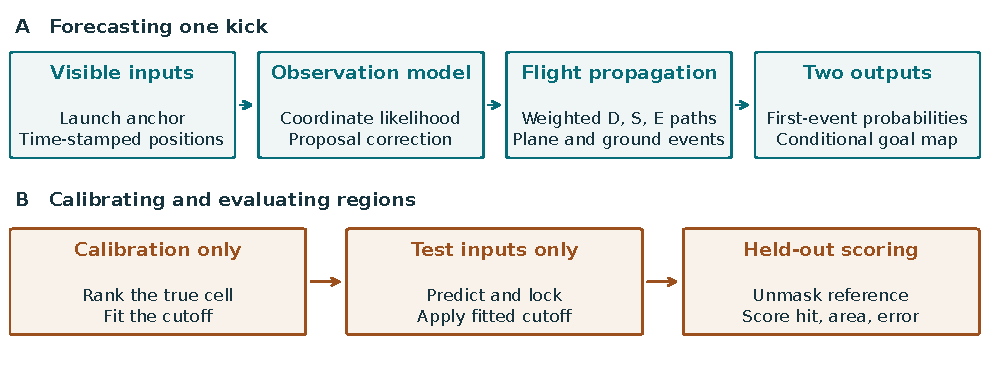
\includegraphics[width=\linewidth]{prediction-workflow.pdf}
\caption{\textbf{From early positions to a forecast.} A follows one kick from its observed positions to first-event probabilities and a location map conditional on direct entry. B shows how we calibrate and test regions on separate kicks (Sec.~\ref{sec:coverage}). Only scoring uses the held-out reference crossings.}
\label{fig:workflow}
\end{figure}

\section{Where the prescribed kick is most likely to cross}

\subsection{Modal cell and joint prediction region}
Conditional on direct entry, the most probable cell contains 29.14\% of the probability (Fig.~\ref{fig:goal}). Its centre, approximately \((Y,Z)=(2.56,2.07)\) m, lies 1.098 m inside the positive-\(y\) post and 0.366 m below the crossbar. The six most probable cells form the rectangle
\begin{equation}
 2.196\le Y\le2.928\ \mathrm{m},\qquad 1.708\le Z\le2.196\ \mathrm{m}.
 \label{eq:region}
\end{equation}
Together these cells occupy \(0.3572\ \mathrm{m^2}\) and contain 90.52\% of the conditional probability. The median crossing time from release is 0.399 s, with 5th and 95th percentiles of 0.392 and 0.407 s.

\begin{figure}[htbp]
\centering
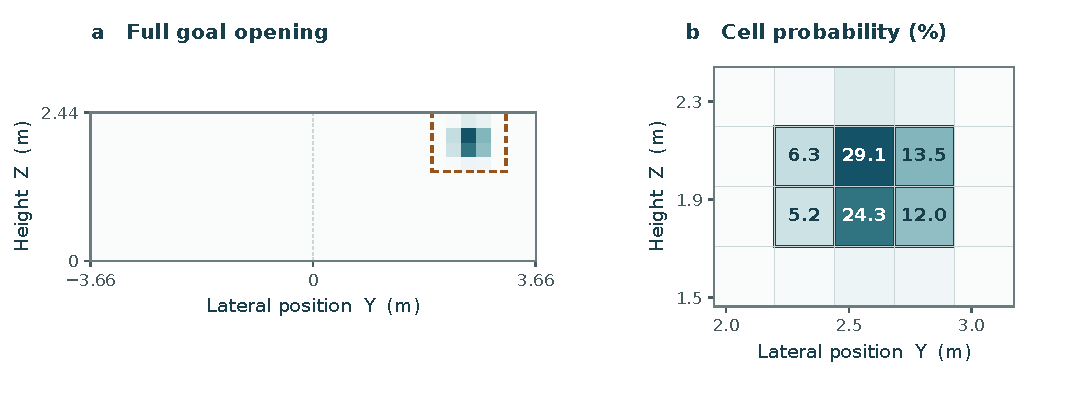
\includegraphics[width=\linewidth]{goal-forecast.pdf}
\caption{\textbf{Predicted location and time of direct entry.} A locates the enlarged area on the goal. B shows the probability per \(0.244\) m square cell using the same colour scale. The outline encloses the six most probable cells and the diamond marks the modal centre. C gives the 5th, 50th and 95th percentiles of the crossing time.}
\label{fig:goal}
\end{figure}

Across two independent runs of 131,072 proposals per model per seed, all 3,469 trajectories with positive weight crossed inside the opening. Thus the estimated direct-entry probability is one under these assumptions and this finite sample. Posterior model weights were \(0,0.346,0.654\) for D, S and E, consistent with the wind bound that excludes D in Eq.~\eqref{eq:wind}. The prescribed kick has no measured crossing or outcome against which to check these estimates.

\subsection{How precisely can the hotspot be located?}
Both seeds selected the cell centred at \((2.562,2.074)\) m. Varying E's share of the combined S/E prior from 10\% to 90\% also preserved this cell. A finer grid moved the modal centre to \((2.501,2.013)\) m, and a half-cell shift of the original grid gave \((2.684,1.952)\) m. The extra digits identify a cell on each grid. The six-cell region in Eq.~\eqref{eq:region} quantifies the nominal spatial uncertainty. The continuous conditional mean, \((2.603,1.970)\) m, minimizes posterior squared distance. Our aerodynamic point forecasts use the centre of the cell with greatest probability at the stated resolution.

The force law also matters over the last eight metres. Fitting launch velocity by least squares under gravity alone gives \((3.217,1.957)\) m. Fitting constant acceleration exactly to release and both frames gives \((2.495,1.920)\) m.


\section{A lower bound on two-position prediction error}
\label{sec:ambig}

\subsection{Two flights consistent with the same observations}
How closely can any point forecast fit every admissible flight? In model S we fixed the wind at zero and \(\beta_x\) at either \(-0.5\) or \(+0.5\ \mathrm{s^{-1}}\). For each choice we fitted the six coordinates at 50 and 100 ms by varying the three launch-velocity components and \(\kappa,\beta_y,\beta_z\). Both fits lie within the prior ranges, with maximum coordinate residual below \(5\times10^{-13}\) m. An independent integration with MATLAB \texttt{ode45} reproduced both crossings~\cite{matlab}.

Both drag coefficients round to \(0.02007\ \mathrm{m^{-1}}\). The fitted \((\beta_y,\beta_z)\) pairs are \((-0.206,-0.463)\) and \((0.085,-0.251)\ \mathrm{s^{-1}}\), respectively. At any instant, a component of \(\vv\beta\) along \(\vv u\) contributes no transverse force. As gravity turns the velocity, that component can influence the later flight. Small adjustments in launch velocity allow different force histories to agree at both early frames.

The two flights yield identical centimetre readings but cross at \(Q_A=(2.57378,2.00251)\) m and \(Q_B=(2.62831,1.93396)\) m, 8.76 cm apart. Any point predictor must give them the same \(\widehat Q\). The triangle inequality then gives
\begin{equation}
 \max\{\norm{\widehat Q-Q_A},\norm{\widehat Q-Q_B}\}
 \ \ge\ \tfrac12\norm{Q_A-Q_B}\ \approx\ 0.0438\ \mathrm{m}.
 \label{eq:witness}
\end{equation}
Thus at least one of the two errors reaches about 4.38 cm whenever both flights are admissible, regardless of their relative frequency.

\begin{figure}[htbp]\centering
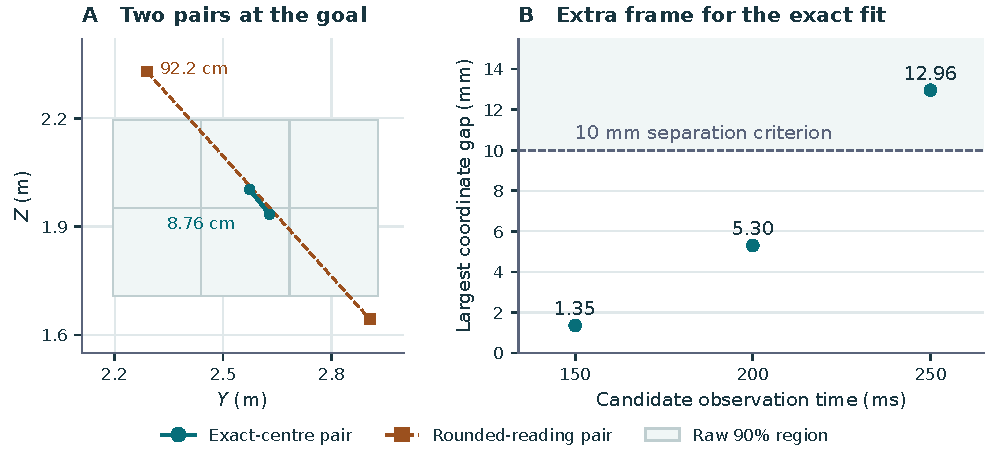
\includegraphics[width=\linewidth]{witness-path.pdf}
\caption{\textbf{Two admissible flights separate after the second reading.} A shows the two model-S crossings with the same scale along both axes. B gives the largest coordinate gap at three candidate observation times. With a 5 mm bound on each coordinate, the reading boxes separate once this gap exceeds 10 mm.}
\label{fig:witnesspath}
\end{figure}

\section{How measurement error affects the forecast}
\label{sec:measurement}

\subsection{Position, timing and rounding errors}
For axis \(a\), let \(d_{ia}\) denote the position in frame \(i\) displayed to the nearest \(q=0.01\) m. We model the displayed value as
\begin{equation}
 d_{ia}=\mathcal R_q\!\left[r_a(t_i+\tau;\theta,M)+b_a+e_{ia}\right],
 \quad b_a\sim N(0,\sigma_b^2),\quad e_{ia}\sim N(0,\sigma_e^2).
 \label{eq:observe}
\end{equation}
Here \(b_a\) is a bias common to the frames of one kick, \(e_{ia}\) is independent across frames and axes, and \(\tau\) shifts all the frame times together. Conditional on \(b,\tau\), the probability of the displayed readings is
\begin{equation}
 L=\prod_{i,a}\left[
 \Phi\!\left(\frac{d_{ia}+q/2-r_a(t_i+\tau)-b_a}{\sigma_e}\right)
 -\Phi\!\left(\frac{d_{ia}-q/2-r_a(t_i+\tau)-b_a}{\sigma_e}\right)\right].
 \label{eq:likelihood}
\end{equation}
Here \(\Phi\) is the standard normal cumulative distribution function. With rounding alone, \(L\) is the indicator that every coordinate lies in its interval. We integrate over \(b\) by sampling from its prior and, for a uniform timing offset on a bounded interval, over \(\tau\) by five- or seven-node Gauss--Legendre quadrature with the same total proposal budget. The synthetic tests prescribe these error distributions.

A position error small enough to miss by eye can dominate the inferred acceleration. For an exact release coordinate and frame errors on one axis with common variance \(\sigma^2\) and correlation \(\rho_e\), the acceleration error inferred from the second difference at spacing \(h\) has variance
\begin{equation}
 \operatorname{Var}\!\left(\frac{e_2-2e_1}{h^2}\right)
   =\frac{(5-4\rho_e)\sigma^2}{h^4}.
 \label{eq:noise}
\end{equation}
A common timing shift contributes \(-v\tau/h^2\) to the acceleration inferred from uniform motion. At \(v=30\) m/s and \(h=50\) ms, a 1 ms shift produces an apparent acceleration of 12 m/s\(^2\). A spatial bias cancels from the second difference if it affects release and both frames equally. If the release coordinate is exact, a bias shared only by the two frames survives and can resemble aerodynamic curvature.

\subsection{Sensitivity of the prescribed forecast}
We varied one assumption at a time in fourteen scenarios and refitted the same readings, using the nominal two seeds and 131,072 proposals per model per seed. Table~\ref{tab:sensitivity} and Fig.~\ref{fig:sensitivity} use displacement of the continuous conditional mean to track movement independently of the grid. Region areas use the original grid.

\begin{table}[htbp]
\centering\small
\caption{Changes from the nominal forecast under individual assumptions. Shift is the distance between continuous conditional means. Area is the raw 90\% region. Changing ball mass affects the force-to-mass factor in E. D and S use fitted acceleration coefficients.}
\label{tab:sensitivity}
\begin{tabular}{@{}lrr@{}}\toprule
Changed assumption & Mean shift (cm) & Area (m\(^2\))\\\midrule
\csname @@input\endcsname tables/sensitivity.tex
\bottomrule\end{tabular}
\end{table}

\begin{figure}[htbp]\centering
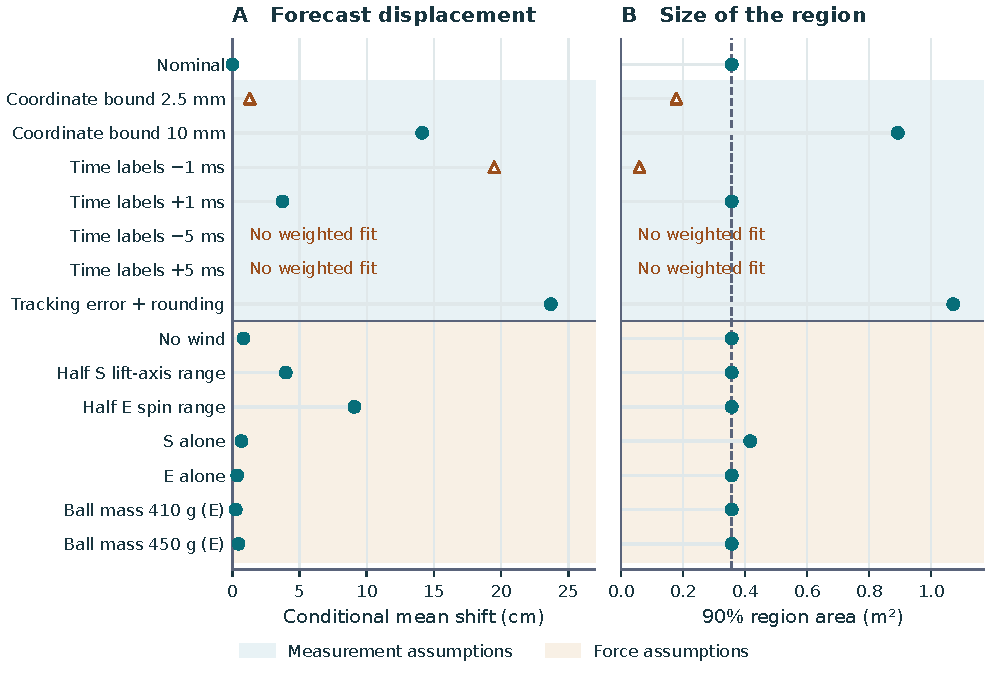
\includegraphics[width=\linewidth]{sensitivity.pdf}
\caption{\textbf{How the expected crossing and region size change.} A shows displacement of the conditional mean. B shows the raw 90\% region area and its nominal value (dashed). Shading identifies observation scenarios. Open triangles mark ESS below the prescribed-case threshold of 200. Rows with zero positive weight have no estimate.}
\label{fig:sensitivity}\end{figure}

Doubling the coordinate bound to 10 mm moves the mean by 14.1 cm and expands the region to \(0.893\ \mathrm{m^2}\). With 6 mm independent tracking error and 8 mm shared bias before rounding, the mean shifts 23.7 cm. On the same grid the most probable cell now lies at \((3.294,1.830)\) m and the raw region covers \(1.072\ \mathrm{m^2}\). Removing wind shifts the mean by 0.83 cm for this kick. Halving E's spin range shifts it by 9.08 cm. The 410--450 g scenarios use the endpoints of the match-ball mass range~\cite{ifab} while holding radius fixed.

A tighter 2.5 mm coordinate bound leaves ESS 68, below the prescribed-case threshold of 200. Moving both observations 1 ms earlier leaves ESS 1. A 5 ms shift in either direction produces no positive-weight samples. These draws give too little support to locate the crossing reliably. Varying one factor at a time also leaves interactions among timing, noise, wind and spin unresolved.


\reserveheadroom
\section{What the 50 ms reading adds at 100 ms}
\label{sec:coverage}

\subsection{Paired forecasts at a common deadline}
At 100 ms both aerodynamic predictors know the latest ball position. We give one of them the 50 ms reading as well. Both start computing at 100 ms with the same priors, force laws and solver. Each draws 8,192 proposals per force model, propagates up to 512 positive-weight samples per model and reports the centre of the most probable goal cell. A gravity-only control uses both readings, predicts a continuous ballistic crossing and assigns direct entry a probability of zero or one.

We generated 90 calibration kicks and 120 test kicks with fresh random seeds. The reference solver used a 1 ms step and different force laws from the predictor, with balanced blocks of zero-spin, stable-spin and low-spin wake trajectories (Appendix~\ref{app:reference}). We calibrated the regions on 55 direct entries and scored locations on the 71 test entries. All 120 test kicks contributed to the event scores.

We rounded each kick's exact coordinates to the nearest centimetre. For a second set of readings, we first added independent Gaussian errors in each frame (6 mm standard deviation per coordinate) and a Gaussian bias shared by both frames (8 mm standard deviation per coordinate). Release position and frame times were exact in both sets. For noisy readings the predictor used the same error model as the generator. Appendix~\ref{app:event} treats timing errors separately.

We prespecified the three methods, coverage targets from 50 to 100\% (90\% for the main comparison), and subgroups by spin family and distance from the goal edge. Each kick used one inference seed across methods and measurement conditions. The predictor saw only the input positions. We saved and hashed its forecasts before scoring them against the references.

\subsection{Calibrating regions on the goal grid}
For each method and measurement condition, calibration sets a threshold for including cells. In the aerodynamic forecasts, rank the grid cells \(j_1,\ldots,j_J\) by decreasing probability \(H_D(j)\) conditional on direct entry, breaking ties in a fixed order. The score of an occupied cell is the mass of the cells ahead of it,
\begin{equation}
 S_D(j_k)=\sum_{\ell<k}H_D(j_\ell).
 \label{eq:coverage-prefix}
\end{equation}
An empty cell scores one. For gravity, a cell whose centre lies distance \(d_j\) from the ballistic crossing scores \(d_j/(L+d_j)\), where \(L\) is the goal diagonal. Thresholding this score amounts to choosing a radius about the crossing. If the map or ballistic crossing is unavailable, every cell receives a score of one.

For a target coverage \(c\), sort the scores of the 55 true calibration cells and take the \(\lceil(55+1)c\rceil\)-th smallest as \(q_c\). Include all cells with \(S_D(j)\le q_c\). If the rank exceeds 55, set \(q_c=1\). Whenever \(q_c=1\), the region covers the whole goal. This split-calibration rule gives marginal coverage under exchangeability~\cite{lei}. Our test measures the hit rate on the specified, block-balanced synthetic population. Coverage on real kicks requires independent field data.

\begin{table}[htbp]
\centering\small
\caption{Forecasts at the 90\% calibration target. Hits, mean area and mean point error use the 71 direct entries. The Brier score for direct entry uses all 120 test kicks. The gravity control uses both readings and a calibrated radius.}
\label{tab:z09main}
\begin{tabular}{@{}llrrrr@{}}\toprule
Profile & Forecast & Hits & Area (m\(^2\)) & Mean error (m) & Brier\\\midrule
\csname @@input\endcsname tables/coverage-main.tex
\bottomrule\end{tabular}
\end{table}

\begin{figure}[htbp]\centering
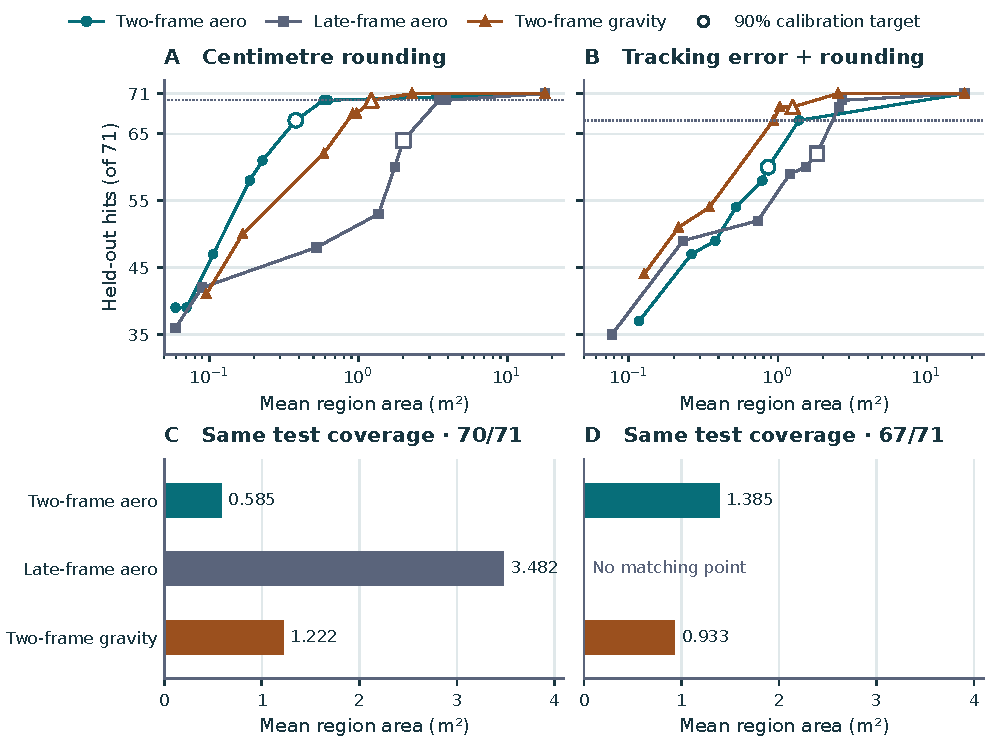
\includegraphics[width=\linewidth]{coverage-frontier.pdf}
\caption{\textbf{Goal area at matched test coverage.} Panels A and B plot hits against mean area on a log scale for the same 71 direct entries. Open markers denote the 90\% calibration target. Panels C and D compare prespecified thresholds that yielded equal hit counts. The late-frame curve has no sampled point at 67/71 hits. The full opening spans \(17.86\ \mathrm{m^2}\).}
\label{fig:frontier}
\end{figure}

\subsection{The early frame narrows the region under centimetre rounding}
At the 90\% target, two frames covered 67/71 entries in \(0.381\ \mathrm{m^2}\) on average, compared with 64/71 in \(2.003\ \mathrm{m^2}\) using the late frame alone (Table~\ref{tab:z09main}). The respective 95\% Wilson intervals for coverage were 86.4--97.8\% and 81.0--95.1\%. At their 95\% targets, both methods covered 70/71 entries. The two-frame region averaged \(0.585\ \mathrm{m^2}\), compared with \(3.482\ \mathrm{m^2}\) for the late frame. Gravity covered 70/71 in \(1.222\ \mathrm{m^2}\) at its 90\% target (Fig.~\ref{fig:frontier}). Equal counts can include different kicks.

Adding the early frame lowered point error on 13 entries, left it unchanged on 54 and raised it on four (Fig.~\ref{fig:paired-error}). The mean reduction was 3.80 cm (95\% interval 0.22--7.62 cm from 4,000 paired resamples of kicks). The mean reduction relative to gravity had a 95\% interval of \(-2.29\) to \(5.85\) cm. The Brier score for direct entry was 0.018 with both frames, 0.070 with the late frame and 0.083 for the binary gravity forecast.

\subsection{Tracking error changes which forecast is more precise}
At the same 90\% target, the two-frame region was the smallest but covered only 60/71 noisy crossings, compared with 62/71 for the late frame and 69/71 for gravity. All eleven misses by the two-frame forecast came from the stable-spin group (12/23 hits). It covered 24/24 in each of the zero-spin and wake groups. Gravity covered 21/23 stable-spin entries (Table~\ref{tab:subgroup}).

At 67/71 observed hits, gravity used \(0.933\ \mathrm{m^2}\) at its 80\% target and two-frame aerodynamics used \(1.385\ \mathrm{m^2}\) at its 95\% target. These two targets yielded equal coverage on this particular test sample. For the 71 direct entries, the aerodynamic grid centre had a mean point error 5.57 cm larger than the continuous gravity forecast (paired 95\% interval 1.17--10.25 cm). The intervals for both the point-error and Brier-score differences between two-frame and late-frame aerodynamics included zero.

Estimating acceleration from the readings divides the second position difference by \(h^2\), with \(h=50\) ms. A bias shared by the two frames survives in that difference when the release position is fixed independently (Eq.~\eqref{eq:noise}). Gravity fixes the acceleration. Its relative precision here is consistent with the difficulty of estimating transverse curvature from noisy readings, even when the noise model is known.

\begin{figure}[htbp]\centering
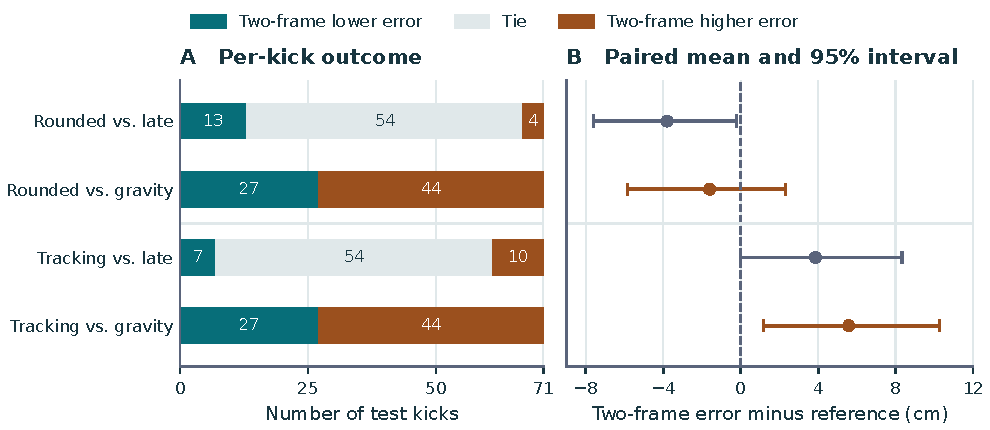
\includegraphics[width=\linewidth]{paired-error.pdf}
\caption{\textbf{Point errors on the same 71 direct-entry kicks.} A counts kicks on which two-frame aerodynamics has a smaller, equal or larger error than each comparison method. B shows the mean paired difference and its 95\% shot-bootstrap interval. Negative values favour two-frame aerodynamics.}
\label{fig:paired-error}
\end{figure}

\subsection{Forecast availability and computation time}
Each method produced a point for all 71 direct entries and an event probability for all 120 kicks under both measurement conditions. Only one run, a noisy late-frame forecast, fell below 25 effective samples. Even with a defined point, the noisy two-frame region filled the entire goal at its 97.5\% target. Appendix~\ref{app:operating} gives the counts near the goal edge.

In the local Python run, two-frame inference and goal-map construction took 84 ms at the median and 94 ms at the 95th percentile with rounding alone. With tracking errors the times were 121 and 131 ms. At the test sampling budget, 131 ms is about 44\% of the nominal 299 ms remaining after the last reading. Capture, reconstruction, transfer and goalkeeper movement require additional time, and the crossing time varies by kick.


\section{From a crossing forecast to a decision time}
For the prescribed kick, the median arrival of 0.399 s leaves 299 ms after the last frame for both computation and movement. In a separate synthetic test, shifting the two observations from 50/100 to 100/150 ms reduced mean point error from 0.182 to 0.126 m and left 50 ms less time to act. Keeping all three frames at the later deadline gave more low-ESS forecasts (Appendix~\ref{sec:waiting}). To translate either forecast into a save probability, one would also need the goalkeeper's initial position, movement onset and reach.

Match tracking poses a different obstacle. Three penalties recorded at 25 Hz had later crossing references, but none had an independently verified release time. The nominal force and measurement assumptions could not explain both early frames in any case. Only one late-frame estimate could be scored retrospectively (Appendix~\ref{app:field}).

The forecast describes an uninterrupted flight under specified aerodynamic priors. Ground rebounds, interventions and collisions with the posts or crossbar could change the outcome near the goal edges, and the mix of forces in actual matches may differ from the synthetic population. The grid, measurement model and decision time therefore belong alongside any quoted point and region.

\section*{Conclusion}
\addcontentsline{toc}{section}{Conclusion}
For the prescribed kick, the nominal modal cell lies at \((Y,Z)\approx(2.56,2.07)\) m. Conditional on direct entry, six cells spanning \(2.196\)--\(2.928\) m laterally and \(1.708\)--\(2.196\) m vertically contain 90.52\% of the model probability over \(0.3572\ \mathrm{m^2}\). Even flights that agree with both early readings can cross 8.76 cm apart.

The 50 ms reading adds most to the forecast when the measurements resolve curvature. Under rounding alone, both aerodynamic forecasts covered 70 of 71 synthetic entries; the two-frame model used much less area. With the specified tracking errors, gravity used less area than two-frame aerodynamics at 67 of 71. Whether either result carries over to match play requires independent measurements of release timing, tracking accuracy and the crossing itself.

\appendix
\section{Timing and coordinate errors at the crossing event}
\label{app:event}

\subsection{Closed-form control and event projection}
With a fixed launch position and readings at \(h\) and \(2h\), the constant-acceleration interpolant uses
\begin{equation}
 \widehat{\vv a}=\frac{\vv r_2-2\vv r_1+\vv r_0}{h^2},
 \qquad
 \widehat{\vv v}_0=\frac{\vv r_1-\vv r_0}{h}
                         -\frac{h}{2}\widehat{\vv a}.
\end{equation}
For the prescribed readings this yields \((30.4,9.4,6.9)\) m/s and
\((-16,-16,-12)\) m/s\(^2\). This is a kinematic diagnostic. It assumes constant acceleration beyond the observations. Write \(X=11-x_0\), \(D=v_{0x}^2+2a_x X\), and assume a positive, transversal first forward root. A numerically stable evaluation is
\begin{equation}
 T=\frac{2X}{v_{0x}+\sqrt{D}},\quad
 \dot{x}(T)=\sqrt{D}.
\end{equation}
The nominal values are \(T=0.4050\) s and \((Y,Z)=(2.495,1.920)\) m. Equation~\eqref{eq:region} is obtained from the aerodynamic inference rather than this control.

Suppose an input perturbation changes the interpolated curve at fixed \(T\) by
\(\delta\vv r(T)\). Differentiating the event condition \(x(T)=11\) gives
\begin{equation}
 \delta T=-\frac{\delta x(T)}{\dot{x}(T)},\qquad
 \delta Q=P\,\delta\vv r(T),\qquad
 P=\begin{pmatrix}
 -\dot y(T)/\dot x(T)&1&0\\
 -\dot z(T)/\dot x(T)&0&1
 \end{pmatrix}.
 \label{eq:event-project}
\end{equation}
This expression converts longitudinal errors into lateral and vertical errors by the local slope of the path. A perturbation parallel to the local velocity changes the time to first order and cancels out of \(Q\). Near \(\dot x(T)=0\) the derivative can grow without bound, and when the forward root disappears the linearized location is undefined.

Let \(s=T/h\), \(\lambda_1=s(2-s)\), and \(\lambda_2=s(s-1)/2\). These are the Lagrange weights of the two observed positions when the launch anchor is fixed. With spatial errors \(\vv e_i\) and a shared true time shift \(\tau\) relative to the time labels, the first-order event shift is
\begin{equation}
 \delta Q=P\left[\lambda_1\vv e_1+\lambda_2\vv e_2+
        \bigl(\lambda_1\vv v(h)+\lambda_2\vv v(2h)\bigr)\tau\right].
 \label{eq:timing-spatial}
\end{equation}
At the nominal root the weights are \(-49.41\) and \(28.76\). Independent 5 mm per-axis bounds contribute first-order shifts of at most 0.439 m in \(Y\) and 0.424 m in \(Z\). A common 1 ms offset contributes \((-0.123,-0.093)\) m for positive offset under the stated sign convention. Central differences at \(1\,\mu\)s reproduce the timing derivative to within \(2\times10^{-5}\) m/s. The large values characterize extrapolation by an unconstrained quadratic. The main model restricts curvature through force and launch ranges.

\subsection{Joint perturbations and loss of a forward root}
For each timing bound and spatial bound, evaluate both phase endpoints and zero phase, and the corners of the six-coordinate box. A zero bound uses one value rather than repeating identical inputs. Refit the polynomial and solve the forward plane event for each case. Ground and goal-edge events are disabled in this diagnostic to isolate the existence of a forward plane root. The maximum shift is taken over tested roots only. A nonlinear map can attain its extrema away from the sampled corners, so this maximum is a scenario statistic.

\begin{table}[htbp]\centering\small
\caption{Joint timing and position stress test for the quadratic control. First-order maxima are coordinatewise sums of absolute derivative contributions. The sampled maximum is a Euclidean shift at a forward plane root. Counts include all selected timing and spatial combinations.}
\label{tab:plane-sens}
\begin{tabular}{@{}rrrrrr@{}}\toprule
Phase bound & Spatial bound & First-order \(Y\) & First-order \(Z\) & Sampled shift & No root\\
(ms) & (mm) & (m) & (m) & (m) & (count)\\\midrule
\csname @@input\endcsname tables/plane-sensitivity.tex
\bottomrule\end{tabular}
\end{table}

The quadratic can lose its plane crossing at a 3 ms timing bound. At 1 ms and 5 mm, all 192 combinations cross and the largest sampled displacement is 0.930 m. The corresponding coordinatewise linear bounds are 0.562 and 0.517 m. Larger perturbations change the root substantially, making the local derivative a poor global description. The different failure counts across spatial bounds reflect the changing discrete corners, not a monotone probability of failure. This is a reason to carry event uncertainty through the solver when propagating input uncertainty. A fixed-time error band alone cannot represent event loss.

\begin{figure}[htbp]\centering
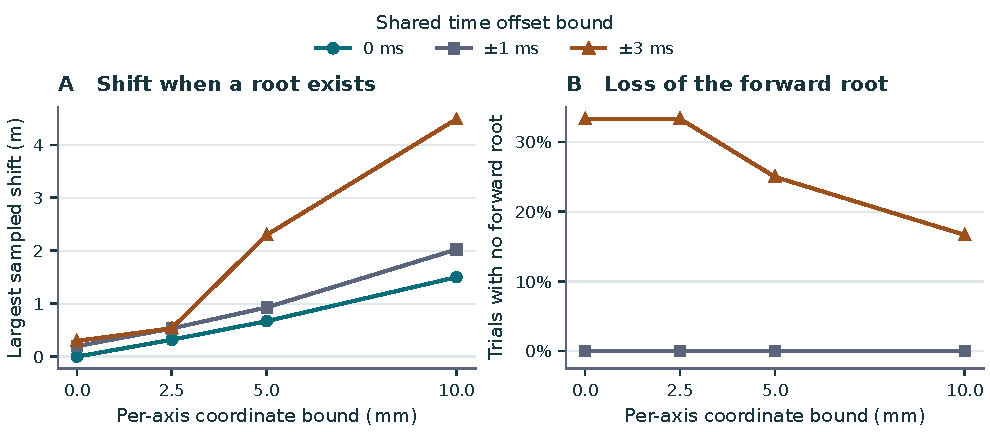
\includegraphics[width=\linewidth]{event-sensitivity.pdf}
\caption{\textbf{Input perturbations can move or remove the forward crossing.} A measures the maximum displacement among sampled corners with a root in the quadratic control. B reports the fraction of enumerated combinations without a root. These are deterministic trial fractions for the stated timing endpoints and position corners. The diagnostic considers the plane alone.}
\label{fig:event-shift}
\end{figure}

\subsection{Covariance propagation for correlated measurements}
Under independent coordinate noise with covariance \(\Sigma_e\) in each frame, a shared bias covariance \(\Sigma_b\), and an independent phase variance \(\sigma_\tau^2\), write \(w=\lambda_1\vv v(h)+\lambda_2\vv v(2h)\). The first-order covariance is
\begin{equation}
 \operatorname{Cov}(\delta Q)=
 P\left[(\lambda_1^2+\lambda_2^2)\Sigma_e+
        (\lambda_1+\lambda_2)^2\Sigma_b+
        \sigma_\tau^2 ww^\top\right]P^\top.
\end{equation}
The timing contribution is rank one. Its direction depends on the trajectory and event geometry. If a common coordinate translation were applied to release and frames alike, its effect would differ because the launch position would also change. The model uses an independently specified launch position. This formula separates local measurement amplification from model discrepancy and Monte Carlo variability. It is valid for a smooth forward crossing away from event switches.

\section{Operating points, subgroups and timing records}
\label{app:operating}
The operating points below report sample counts instead of treating calibration targets as test guarantees. Mean area includes every true direct entry. At a target of one the entire rectangular opening is returned by construction.

\begin{table}[htbp]\centering\small
\caption{Selected calibration targets and realized results from the 120-kick holdout. Rounded and tracking profiles share the 71 true direct entries.}
\label{tab:coverage-full}
\begin{tabular}{@{}llrrr@{}}\toprule
Profile & Forecast & Target (\%) & Hits & Mean area (m\(^2\))\\\midrule
\csname @@input\endcsname tables/coverage-targets.tex
\bottomrule\end{tabular}
\end{table}

\begin{table}[htbp]\centering\small
\caption{Hits at the 90\% calibration target by generator family and distance to the opening edge. The two edge strata partition direct entries. The three family strata form a separate partition. They are descriptive and were not separately calibrated.}
\label{tab:subgroup}
\begin{tabular}{@{}llrrrr@{}}\toprule
Profile & Stratum & Entries & 100 ms & 50 + 100 ms & Gravity\\\midrule
\csname @@input\endcsname tables/coverage-strata.tex
\bottomrule\end{tabular}
\end{table}

Near-edge means the minimum distance from the true direct entry to any of the four edges is below 0.244 m, the nominal cell width. The strata expose whether a successful overall average masks failures near the physical decision boundary. Family is available for evaluation only. The predictor never receives the synthetic truth label.

\begin{table}[htbp]\centering\small
\caption{Numerical availability and wall-clock timing in a single local run. Runtime includes inference and construction of the predicted region ranking inputs. The ballistic timing covers its trajectory result. Threshold application is omitted in both. Times are descriptive for this host and software environment.}
\label{tab:runtime}
\begin{tabular}{@{}llrrrrr@{}}\toprule
Profile & Forecast & Points & Events & ESS \(<25\) & Median (ms) & 95th (ms)\\\midrule
\csname @@input\endcsname tables/coverage-runtime.tex
\bottomrule\end{tabular}
\end{table}

The benchmark has one seed for each shot and profile. Paired intervals use 4,000 resamples of differences matched by shot ID. Event intervals use all shots. Position, area and hit intervals use the true direct entries. The test is balanced by generator family before observing outcomes. Intervals are descriptive of the sampled mixture. An independent field calibration would need known release, independent reference crossings, and an explicit protocol for intervening contacts.

\section{Implementation and physical checks}
\label{app:algorithm}
\subsection{A callable forecast contract}
The general method accepts the release point, a list of observed positions and timestamps, a camera-error model, and documented parameter supports. Input indices must be valid and coordinates finite. The solver advances each hypothesis from release to the last observation, rejecting a path that contacts the ground before the observations. Integrate surviving hypotheses until the earliest goal-plane crossing, descending ground contact, or horizon. The goal-plane coordinates are attached to an entry only when they lie in the open goal rectangle.

\begin{enumerate}
\item For each force family, sample wind and spin parameters. Form a launch-velocity proposal around the inversion of the last observation. Keep a 2\% prior draw to provide support away from the local proposal.
\item Evaluate the observation likelihood at all supplied times and assign importance weights as in Eq.~\eqref{eq:weights}. If including a timing nuisance, distribute the fixed budget over quadrature nodes and combine their masses with the node weights.
\item Carry posterior mass to first events. For each crossing through the goal, assign its weight to a fixed cell. Normalize the event masses using the total weight and normalize goal-cell masses using the entry weight.
\item Return the event vector, modal cell, raw region and effective sample size. Report an unavailable event distribution when total mass is zero. If total mass is positive but entry mass is zero, report the event distribution and mark the conditional point and map undefined.
\end{enumerate}

This separation avoids conflating a missed goal with an unsupported forecast. A boundary case can have a computed event vector and very little entry mass, so a conditional point should be accompanied by the unconditional entry probability. The physical support test and the numerical ESS warning answer separate questions.

\subsection{Model assumptions and checks}
\begin{table}[htbp]\centering\small
\caption{Roles of inputs in the nominal prediction. Changes to scenario choices require a fresh forecast.}
\label{tab:assumptions}
\begin{tabular}{@{}p{.31\linewidth}p{.24\linewidth}p{.36\linewidth}@{}}\toprule
Quantity & Role & Interpretation\\\midrule
Release, frame times, and opening & Given by the problem & Geometry and information budget\\
Ball mass, radius and air density & Nominal physical inputs & Set acceleration through the area-to-mass factor\\
Empirical drag curve & Literature-guided law & Limited range, with clipping and an offset prior\\
Wind and lift/spin bounds & Scenario and prior choices & Control admissible continuations and model weights\\
5 mm coordinate interval & Nominal rounding assumption & Relates reported positions to continuous paths\\
Cell resolution and RK4 steps & Numerical choices & Check stability before quoting modal coordinates\\
6 mm noise and 8 mm bias & Synthetic test parameters & Specify a noisy measurement regime\\
\bottomrule\end{tabular}
\end{table}

In the no-drag, no-lift limit, \(x(t)=v_{0x}t\), \(y(t)=v_{0y}t\), and \(z(t)=R+v_{0z}t-gt^2/2\). This gives closed-form plane and ground times and checks event ordering in the integrator. Under still-air drag without lift, both horizontal acceleration components are proportional to the corresponding velocity components, so the horizontal heading remains fixed. The constant-wind criterion in Eq.~\eqref{eq:wind} generalizes this relation in the wind frame. These limits check geometry and force signs independently of the posterior sampling.

For numerical cross-checks, the existing RK4 comparisons against adaptive DOP853 cover vacuum, drag with ground contact, effective lift and the speed-dependent empirical law. The largest reported event-position difference is 0.171 mm and the largest event-time difference is 0.038 ms. These four checks establish local numerical agreement under specified force laws. A finer solver cannot identify unknown wind, spin, or release-time error. The witness pair uses its own high-accuracy integration and a separate MATLAB replay.


\section{Reference flights and earlier synthetic tests}
\label{app:reference}
\label{sec:tests}

\subsection{The reference generator and kinematic controls}
To test how the forecast responds to imperfect force laws, we generated reference flights with a different drag curve,
\[
 C_D^{\rm ref}=0.19+\frac{0.20}{1+\exp[(U-20)/2.5]}+d_0,
 \qquad d_0\sim\mathcal U(0,0.1),
\]
and a lift coefficient \(0.32\tanh(4R\norm{\vv\omega\times\vv u}/U^2)e^{-0.12t}\) acting along \(\vv\omega\times\vv u\). Launch-velocity components were independently uniform on \([20,36]\), \([-11,11]\), \([2,10]\) m/s. Wind was uniform on a horizontal disk of radius 2.5 m/s. We used equal numbers of kicks with zero spin, stable spin and a low-spin wake. Their spin-component bounds were 0, 55 and 6 rad/s. Wake flights also had a time-varying acceleration given by projecting \(A(0,\sin\phi(t),0.4\cos\phi(t))\) perpendicular to \(\vv u\). We chose \(A\in[2,5]\) m/s\(^2\), a period of 0.18--0.55 s and a uniform initial phase. Experiments motivate including unsteady low-spin forces~\cite{mizota}. The amplitudes, periods and family proportions here are synthetic.

The original study used DOP853~\cite{scipy} and split whole kicks into 9 for development, 36 for calibration and 48 for blind testing. Later tests used new seeds with the same reference generator and a 1 ms RK4 step. On the original 48 DOP853 flights, RK4 reproduced every first event, with maximum differences of \(1.9\times10^{-6}\) m at the crossing and \(6.3\times10^{-7}\) s in event time. We gave each predictor only its designated early frames and saved and hashed its forecasts before scoring. These comparisons test numerical agreement and performance on the simulated kick population.

On true direct entries we report Euclidean point error, region hits and mean region area. We score the probability of direct entry across first events with the Brier score \((P(G)-\mathbf1_G)^2\). We compare against a least-squares fit under gravity alone and a constant-acceleration fit through the three positions. We count missing event forecasts separately from missing conditional points.

\subsection{The early frame at a fixed sampling budget}
Of the original 48 blind-test kicks, 33 entered directly, ten crossed outside the opening and five hit the ground first. The two-frame method had median point error 0.133 m and raw-region coverage 30/33, using eight times the single-frame proposal budget. We revisited the same kicks with 2,048 proposals per model for each input choice and three paired seeds (Table~\ref{tab:budget}).

\begin{table}[htbp]\centering\small
\caption{Retrospective test at 100 ms with equal proposal budgets. The 33 direct entries and three seeds give 99 point forecasts. Both methods returned event estimates on all 144 attempts. Regions use raw probabilities.}
\label{tab:budget}
\begin{tabular}{@{}lrrrr@{}}\toprule
Observed frames & Mean error (m) & Hits & Area (m\(^2\)) & ESS $<25$\\\midrule
\csname @@input\endcsname tables/equal-budget.tex
\bottomrule\end{tabular}\end{table}

Adding the 50 ms reading narrowed the regions and reduced their coverage. We averaged paired differences over seeds within each kick, then resampled the 33 kicks 2,000 times. The mean point-error difference (both frames minus the late frame) was \(-4.46\) cm, with a descriptive 95\% bootstrap interval of \([-9.14,0.08]\) cm. The equal-budget result supports a reduction in area. The interval still admits zero improvement in mean point error.

\subsection{When tracking noise exceeds the rounding interval}
We applied three likelihoods to identical noisy positions on a separate set of 36 calibration and 48 test kicks. Before centimetre rounding we added an 8 mm Gaussian bias shared across frames for each axis and independent 6 mm Gaussian frame errors. All aerodynamic forecasts used 8,192 proposals per model and two paired seeds. One likelihood treated the combined 10 mm marginal error as independent, one used the simulated 6/8 mm decomposition, and one allowed only rounding. The two tracking models used a local velocity-proposal half-width of \(0.026\,\mathrm{m}/t\). The rounding-only model used \(0.007\,\mathrm{m}/t\). Importance weights corrected each proposal. The finite-budget comparison therefore includes both the likelihood and the proposal width.

\begin{table}[htbp]\centering\small
\caption{Noisy-input tests at 100 ms on 36 direct entries and two seeds. \(n_Q\) counts available point forecasts. Region hits and mean area use all 72 attempts. An undefined map gives an empty raw region. A calibrated region can encompass the whole opening.}
\label{tab:noise}\setlength{\tabcolsep}{4pt}
\begin{tabular}{@{}lrrrrrr@{}}\toprule
 & Mean error & $n_Q$ & Raw & Raw area & Calibrated & Cal. area\\
Likelihood & (m) & & hits & (m\(^2\)) & hits & (m\(^2\))\\\midrule
\csname @@input\endcsname tables/noise.tex
\bottomrule\end{tabular}\end{table}

We calibrated each method and seed separately using the prefix-mass score in Sec.~\ref{sec:coverage}. A true cell with zero mass receives score one. With \(n\) calibration entries, we include every cell whose score is at most the \(\lceil0.9(n+1)\rceil\)th ordered calibration score. A cutoff of one or a rank above \(n\) returns the whole opening. Coverage is empirical here because the design balances synthetic families and the field error distribution is unknown.

The rounding-only method covered all 72/72 entries after calibration by returning the entire \(17.861\ \mathrm{m^2}\) goal. The shared-bias likelihood reduced mean point error relative to rounding alone by 15.86 cm on 34 complete paired kicks (95\% shot-bootstrap interval 4.95--26.53 cm). Its interval against the independent-error model includes zero. Gravity had lower mean point error (0.220 m) than either tracking model, but its event Brier score was higher (0.104 versus 0.069 for independent errors and 0.064 for shared bias). The rounding-only Brier score was 0.101 on 94/96 attempts. The other methods supplied all 96 event estimates.


\section{The value and cost of waiting for another frame}
\label{sec:waiting}

\subsection{Moving the last frame or keeping an extra one}
Using these same calibration and test kicks with rounding alone, we compared three sets of observations at 8,192 proposals per model and two paired seeds. Moving from the 50/100 ms pair to the 100/150 ms pair delays the decision. Comparing that later pair with all three frames holds the 150 ms deadline fixed.

\begin{table}[htbp]\centering\small
\caption{Additional observations on 36 direct entries with two seeds (72 attempts). \(n_Q\) counts available point forecasts. An undefined map contributes a miss and zero area. Missing event estimates and low ESS use all 96 attempts.}
\label{tab:waiting}\setlength{\tabcolsep}{4pt}
\begin{tabular}{@{}lrrrrrr@{}}\toprule
Frames (ms) & Mean error & $n_Q$ & Hits & Area & No event & ESS $<25$\\
 & (m) & & & (m\(^2\)) & estimate & \\\midrule
\csname @@input\endcsname tables/waiting.tex
\bottomrule\end{tabular}\end{table}

\begin{figure}[htbp]\centering
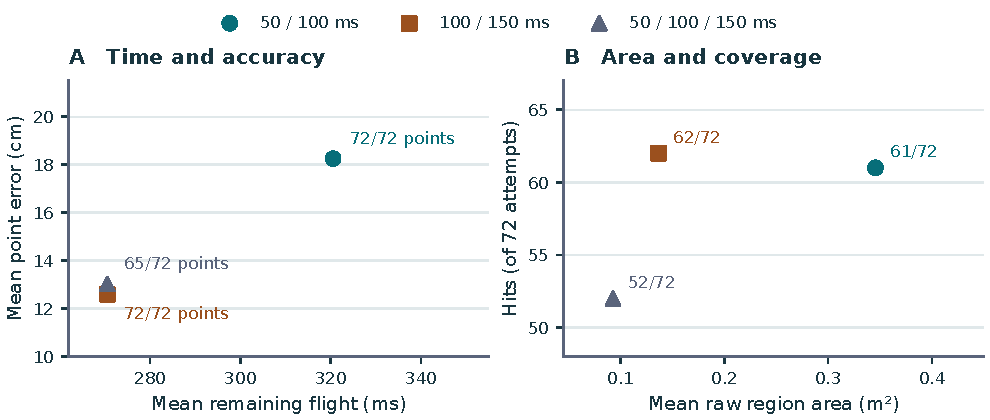
\includegraphics[width=\linewidth]{waiting-tradeoff.pdf}
\caption{\textbf{Forecast accuracy and time left to act.} A shows mean point error for available direct-entry estimates (65/72 for three frames) and mean remaining flight time over all 36 direct entries, before computation or goalkeeper movement. B shows raw region area and coverage, with undefined maps counted as empty (Table~\ref{tab:waiting}).}
\label{fig:waiting}\end{figure}

Waiting for the later pair reduced mean point error by 5.65 cm on 36 complete paired kicks (95\% shot-bootstrap interval 2.79--8.98 cm). Mean time remaining fell from 321 to 271 ms. Calibrated coverage rose from 61/72 to 64/72 while mean area fell from 0.350 to \(0.177\ \mathrm{m^2}\).

At the same 150 ms deadline, keeping all three frames left six of 96 attempts without an event estimate and 46/96 with low ESS. Both seeds yielded paired points on only 31 kicks. On those kicks the three-frame mean point error exceeded the later pair's by 0.27 cm (95\% interval \([-1.71,2.28]\) cm). The three-frame raw regions were smaller but covered only 52/72 entries. Few proposals fit all three readings. This limits what the comparison can establish about the earliest frame's information content. Model error and finite-test variation may also contribute. An adaptive or sequential sampler would need its own validation.

\subsection{When a later frame distinguishes the two fitted flights}
At 150, 200 and 250 ms, the largest coordinate gaps in the pair from Sec.~\ref{sec:ambig} are 1.35, 5.30 and 12.96 mm (Fig.~\ref{fig:witnesspath}B). Deterministic centimetre rounding already gives different heights at 200 ms, 1.26 and 1.25 m. If each coordinate can carry any error within \(\pm5\) mm, the two reading boxes still overlap at that time. Of the three times tested, only 250 ms distinguishes the flights for every allowed error.


\subsection{Which frames reach the predictor in time?}
We simulated 13 camera and noise conditions on a separate set of 48 kicks, 16 per force family and 33 direct entries. At each deadline on the estimated release clock (50 and 100 ms), we selected the latest distinct frame already received and at most 10 ms old. The predictor used its native timestamp. With 2 ms delivery delay, rates of 25, 60, 120 and 240 Hz supplied both readings on 0, 22, 47 and 48 kicks, respectively. At 240 Hz, increasing the delay to 6 ms reduced availability to 46/48. These counts depend on the simulated phase and frame-age rule. Computation takes additional time.

\begin{figure}[htbp]\centering
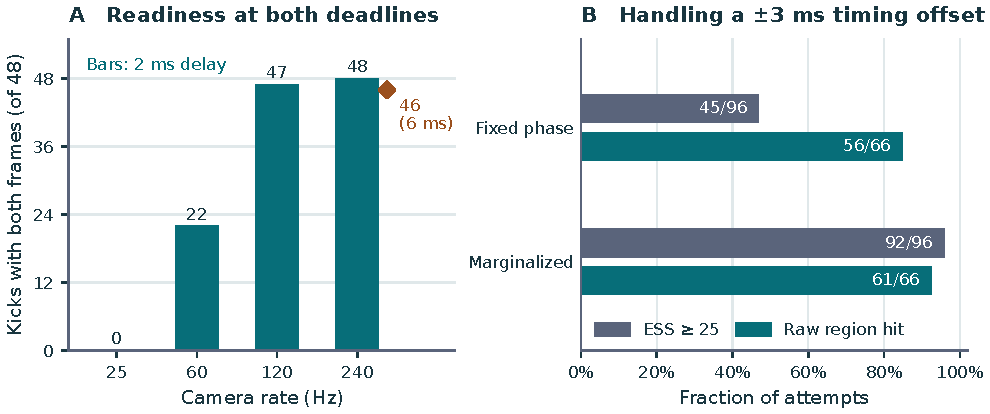
\includegraphics[width=\linewidth]{capture-readiness.pdf}
\caption{\textbf{Timely frames and uncertain release times.} A counts how many of the 48 kicks supplied both frames on time. B compares a fixed release estimate with integration over the simulated \(\pm3\) ms offset. ESS uses 96 attempts (48 kicks and two seeds). Raw-region coverage uses 66 direct-entry attempts.}
\label{fig:capture}
\end{figure}

For periodic frames delivered with fixed delay \(\ell\) and no drops, the oldest possible latest frame has age bounded by \(\ell+1/f\), where \(f\) is the frame rate. To guarantee the 10 ms age limit at 2 ms delivery delay requires at least 125 Hz. A 240 Hz camera allows more margin, but consecutive exposures alone bracket release only to a half-width of about 2.08 ms. A 1 ms timing target would require an independent, finer time reference.

Integrating over the same simulated \(\pm3\) ms release offset increased the number of forecasts with ESS at least 25 from 45/96 to 92/96. Raw regions covered 61/66 entries, up from 56/66. They also grew from 0.377 to \(0.543\ \mathrm{m^2}\) on average, and mean point error rose from 0.196 to 0.218 m. These simulated conditions provide targets for a field trial.


\reserveheadroom
\section{Compatibility with 25 Hz match tracking}
\label{app:field}

\subsection{Reference crossings on the match clock}
The seven matches in the IDSSE v1 elite-soccer dataset contained three executed penalties, all recorded as goals~\cite{bassek}. We translated the longitudinal coordinate by 41.50 m into the penalty-spot frame. We treated the first live frame after a dead-ball interval as an exact anchor and evaluated forecasts at \(+80\) ms using the original priors and a 5 mm coordinate bound. The inputs were either the \(+80\) ms frame alone or the pair at \(+40\) and \(+80\) ms. Reference crossings were interpolated from later frames in the same system, at least 0.32 s after the cutoff. We locked the forecasts before scoring, but had seen the crossings while screening the data.

\begin{table}[htbp]
\centering
\caption{Three penalties on the match clock. The tracked crossing is the reference. The displacement or second difference in the third column yields the required minimum acceleration under the launch assumptions. Here \(\Delta^2x=x_2-2x_1+x_0\).}
\label{tab:field}
\small
\setlength{\tabcolsep}{3.4pt}
\renewcommand{\arraystretch}{1.13}
\begin{tabular*}{\linewidth}{@{\extracolsep{\fill}}lccr@{}}
\toprule
Fixture & Reference \((Y,Z)\) (m) & Observed quantity (m) & Min.\ accel.\ (m/s\(^2\))\\
\midrule
Cologne--Bayern           & \((2.750,0.160)\) & \(z_1-z_0=-0.030\) & 106.25\\
D\"usseldorf--Regensburg  & \((2.919,1.179)\) & \(\Delta^2x=0.510\) & 309.38\\
D\"usseldorf--Kaiserslautern & \((3.070,0.466)\) & \(\Delta^2x=1.100\) & 678.13\\
\bottomrule
\end{tabular*}
\end{table}

\subsection{An acceleration bound for consecutive positions}
In constant wind the energy balance gives \(\dot U\le g\), so \(U\le\sqrt{38^2+12^2+11^2}+3+9.81(0.080)=45.125\) m/s over the first 80 ms. Drag and lift are orthogonal in Eq.~\eqref{eq:acc}. Combining them in quadrature and adding \(g\) gives upper acceleration bounds of 58.681, 89.170 and 102.648 \(\mathrm{m/s^2}\) for D, S and E, using \(C_D\le0.771\) and \(C_L\le0.38\) in E. Thus \(A_*=102.648\ \mathrm{m/s^2}\) bounds all three models.

For three coordinates \(q_0,q_1,q_2\) at spacing \(h=0.040\) s, the true second difference integrates acceleration against a triangular kernel of area \(h^2\). An exact anchor and errors bounded by \(\epsilon\) in the two later positions therefore require
\begin{equation}
 |q_2-2q_1+q_0|\le A_*h^2+3\epsilon,\qquad
 z_1-z_0\ge v_{z,\min}h-\tfrac12 A_*h^2-\epsilon .
 \label{eq:support}
\end{equation}
The second inequality uses the launch prior \(v_{z,\min}=1.5\) m/s. Regensburg's successive \(x\)-increments of 0.71 and 1.22 m require at least \((0.510-0.015)/h^2=309.38\ \mathrm{m/s^2}\). Kaiserslautern's record repeats the anchor and then advances 1.10 m. Cologne misses the vertical bound by just 2.9 mm. All three exceed the common acceleration cap under the assumed launch conditions (Table~\ref{tab:field}).

Treating the anchor as a ball already in flight helps distinguish these failures. Relaxing the lower bound on vertical velocity from \(+1.5\) to \(-11\) m/s gives Cologne two forecasts with ESS 58 and 48. The other two records remain unsupported. Cologne is sensitive to the assumed initial velocity, and its release time remains unknown.

\subsection{A forecast from the late frame alone}
Using only the \(+80\) ms position, neither seed gave positive weight for Cologne or Kaiserslautern. Both placed the Regensburg modal cell at \((2.074,1.098)\) m, 0.849 m from the reference. The first raw region covered \(4.941\ \mathrm{m^2}\) and contained the reference. The second covered \(4.584\ \mathrm{m^2}\). With the same late frame, gravity and straight-line fits missed by 0.809 and 1.219 m. With both frames, gravity missed by 0.853 m at Regensburg and predicted ground contact first in the other two cases.

\begin{figure}[htbp]\centering
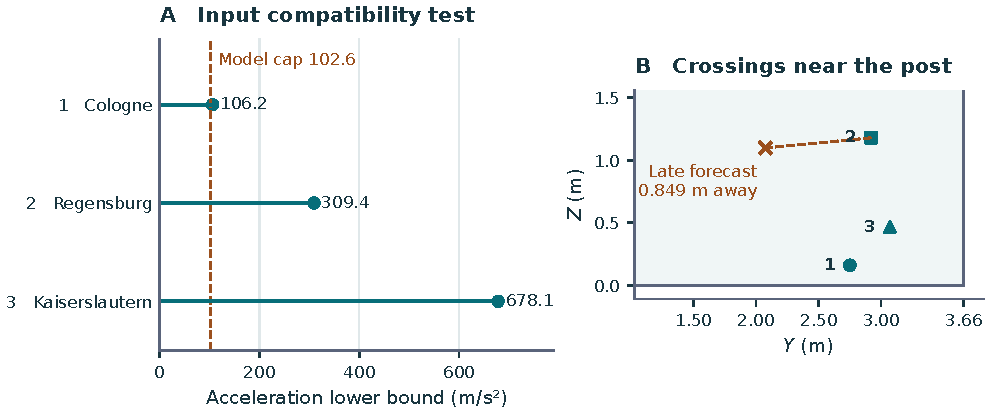
\includegraphics[width=\linewidth]{field-diagnostics.pdf}
\caption{\textbf{Testing the launch assumptions against three match records.} A compares the required minimum accelerations with the common model cap. B locates the three later crossing references near the positive-\(Y\) post. The cross marks the only available late-frame aerodynamic forecast. The records leave release timing and the first event unverified.}
\label{fig:field}
\end{figure}


\section{Evidence needed for a field test}

\subsection{What the available tracking data resolve}
Regensburg's anchor lay about 7 cm horizontally from the penalty spot. The other two anchors were already 0.71 and 1.47 m downfield. No kick had a release time independently verified within 10 ms or a direct entry confirmed as its first event. The acceleration test identifies incompatible inputs and assumptions. It cannot distinguish a mid-flight starting frame from a timing or tracking error. The single scoreable late-frame map gives no estimate of field coverage.

ISSIA-3D provides a separate multi-camera reconstruction of one match sequence~\cite{issia}. Of 79 continuous segments, 61 supplied two positions 80 ms apart and 47 retained the ball for another 120 ms. On those 47, constant-velocity extrapolation gave a median three-dimensional error of 0.162 m. Holding the last position gave 0.996 m. These were subsequent positions in ordinary play. Penalty testing also needs an identified release and a first event at or before the goal plane.

\subsection{A release-synchronized validation protocol}
Independently annotate contact in synchronized multi-view footage and record clock alignment, coordinate calibration, lost frames and intervening contacts. For a scoreable kick, both early positions must be available by the cutoff and the first event must be identifiable. Record interceptions before the natural crossing as contacts or censored outcomes.

Use independent calibration sequences to estimate timing bias, per-axis error and cross-frame dependence in Eq.~\eqref{eq:observe}. The three existing cases can guide development. Freeze the model before testing on held-out matches. Report forecast availability among eligible kicks, point error, joint coverage and area on the same direct entries, and Brier scores on confirmed first events.

The nominal 0.399 s schedule leaves 299 ms after the 100 ms reading and only 149 ms after a 250 ms reading. A field test of additional information such as spin or wind should use the same kicks and count the time needed to obtain each measurement.

\subsection{Scope of the evidence}
The wind inequality and the fitted pair establish limits under specified force and measurement assumptions. Solver comparisons test the integration of those equations. The synthetic holdouts measure how well forecasts transfer to different prescribed force laws. The match records expose conflicts with launch and timing assumptions. Measuring field accuracy still requires independent release and crossing references.

The ball-centre model omits deformation, finite-radius collisions with posts or crossbar, rebounds and goalkeeper contacts. Model weights depend on unmeasured priors and the empirical coefficients need not match the ball. Only the reference generator includes a low-spin wake. One-factor tests leave joint extremes unresolved. Repeated seeds change sampling variability without adding independent kicks. The sampler has been tested offline, and camera readiness alone does not measure end-to-end delivery time.

A forecast should identify its decision time and input frames, report first-event probabilities, and state the point convention and joint region whenever direct-entry mass is positive. Coverage, area, sampling support and the frequency of unavailable forecasts show how much information those outputs carry.

\section{Reproducing the forecasts}
The source archive records the prescribed-case inputs, seeds 8111/8117, the \(30\times10\) grid and solver tolerances. The equal-budget replay uses three seeds. The additional-frame and noise tests use truth seeds 77401/77407 and inference seeds 77501/77507. Tables and figures draw on frozen outputs, with checksums for the benchmark source and predictions. Reproducing the prescribed forecast requires no match data.

\begin{center}\small
\begin{tabular}{@{}ll@{}}\toprule
Claim or check & Package evidence\\\midrule
Wind geometry and model assumptions & \texttt{design/}, \texttt{report/methods.md}\\
Feasible pair and prescribed prediction & \texttt{experiment/runs/B01/}, \texttt{B03/}\\
Equal-budget comparisons & \texttt{experiment/runs/Z04/}, \texttt{report/evidence/z09-replay.zip}\\
Conditional factor sensitivity & \texttt{report/evidence/z05-factors.csv}\\
Timing and noisy-input tests & \texttt{report/evidence/z06-summary.json}\\
Match timing and anchor checks & \texttt{report/field.md}, \texttt{experiment/runs/Z07/}\\
Causal acquisition simulations & \texttt{report/evidence/z08-feedback.csv}\\
Generated tables & \texttt{paper/build\_assets.py}, \texttt{build\_revision\_assets.py}\\
Vector figures and plotted data & \texttt{paper/build\_visuals.py}, \texttt{visual-data.json}\\\bottomrule
\end{tabular}\end{center}

From the repository root, run \texttt{python report/recheck.py}, \texttt{python report/recheck\_field.py} and \texttt{python report/recheck\_extensions.py} for the headline checks. The two table builders and \texttt{python paper/build\_visuals.py} regenerate the assets used by \texttt{paper/manuscript.tex}. The figure builder verifies the goal-cell mass, computes area and coverage from frozen scores, joins point errors by kick and records plotted values and SHA-256 hashes. The scripts \texttt{coverage\_benchmark.py} and \texttt{event\_sensitivity.py} replay the 100 ms test and the crossing-perturbation trials, respectively. The reproduction guide locates their inputs, thresholds and checks.

\begin{thebibliography}{99}\small
\addcontentsline{toc}{section}{\refname}
\setlength{\itemsep}{4pt}
\bibitem{upc}
University Physics Competition, 2026 contest, Problem B.
\href{https://uphysicsc.com/2026contest.html}{Official problem statement}.
\bibitem{goff2010}
J.~E. Goff and M.~J. Carr\'e, Soccer ball lift coefficients via trajectory analysis.
\emph{European Journal of Physics} \textbf{31}, 775--784 (2010).
DOI \doi{10.1088/0143-0807/31/4/007}.
\bibitem{goff2017}
J.~E. Goff, J. Kelley, C. Hobson, K. Seo, T. Asai and S. Choppin,
Creating drag and lift curves from soccer trajectories.
\emph{European Journal of Physics} \textbf{38}, 044003 (2017).
DOI \doi{10.1088/1361-6404/aa6fcd}.
\bibitem{scipy}
P. Virtanen et al., SciPy 1.0: fundamental algorithms for scientific computing in Python.
\emph{Nature Methods} \textbf{17}, 261--272 (2020).
DOI \doi{10.1038/s41592-019-0686-2}.
\bibitem{matlab}
L.~F. Shampine and M.~W. Reichelt, The MATLAB ODE Suite.
\emph{SIAM Journal on Scientific Computing} \textbf{18}, 1--22 (1997).
DOI \doi{10.1137/S1064827594276424}.
\bibitem{mizota}
T. Mizota et al., The strange flight behaviour of slowly spinning soccer balls.
\emph{Scientific Reports} \textbf{3}, 1871 (2013).
DOI \doi{10.1038/srep01871}.
\bibitem{ifab}
International Football Association Board, Laws of the Game, Law 2: The Ball.
\href{https://www.theifab.com/laws/latest/the-ball/}{Ball specifications}, accessed 7 November 2026.
\bibitem{lei}
J. Lei, M. G'Sell, A. Rinaldo, R. J. Tibshirani and L. Wasserman,
Distribution-Free Predictive Inference for Regression.
\href{https://arxiv.org/abs/1604.04173}{arXiv:1604.04173}.
\bibitem{bassek}
M. Bassek, R. Rein, H. Weber and D. Memmert, An integrated dataset of spatiotemporal and event data in elite soccer.
\emph{Scientific Data} \textbf{12}, 195 (2025).
DOI \doi{10.1038/s41597-025-04505-y}. IDSSE v1 data, CC BY 4.0,
DOI \doi{10.6084/m9.figshare.28196177.v1}.
\bibitem{issia}
M. Guti\'errez-P\'erez and A. Agudo, SoccerNet-v3D: Leveraging sports broadcast replays for 3D scene understanding.
\emph{IEEE/CVF CVPR Workshops} (2025). DOI \doi{10.1109/CVPRW67362.2025.00595}.
\href{https://github.com/mguti97/SoccerNet-v3D/releases/tag/v1.0.0}{ISSIA-3D annotations, release 1.0.0}.
\end{thebibliography}

\section*{Report on the Use of AI}
\addcontentsline{toc}{section}{Report on the Use of AI}
OpenAI Codex assisted with the physical analysis, numerical implementation, evidence checks, figure generation and revision of the English manuscript.
\IfFileExists{ai-verbatim.tex}
  {\input{ai-verbatim.tex}}
  {This public draft contains the disclosure only. The complete original prompts and outputs are to be appended to the submission copy from the team's interaction records.}
\end{document}
